\section{Motivation}
\label{sec:motivation}
\label{sec:assumptions}

In this section, we summarize the argument for replacing task-level fault
tolerance as MapReduce's fault tolerance scheme for ``dense'' clusters. We then
provide an overview of alternative fault approaches used by current data
processing systems.

\subsection{Fault Tolerance for ``Dense'' Clusters}
\label{sec:ft_provenance}

\begin{figure*}[t]
\centering
\begin{subfigure}[t]{0.47\textwidth}
  \centering
  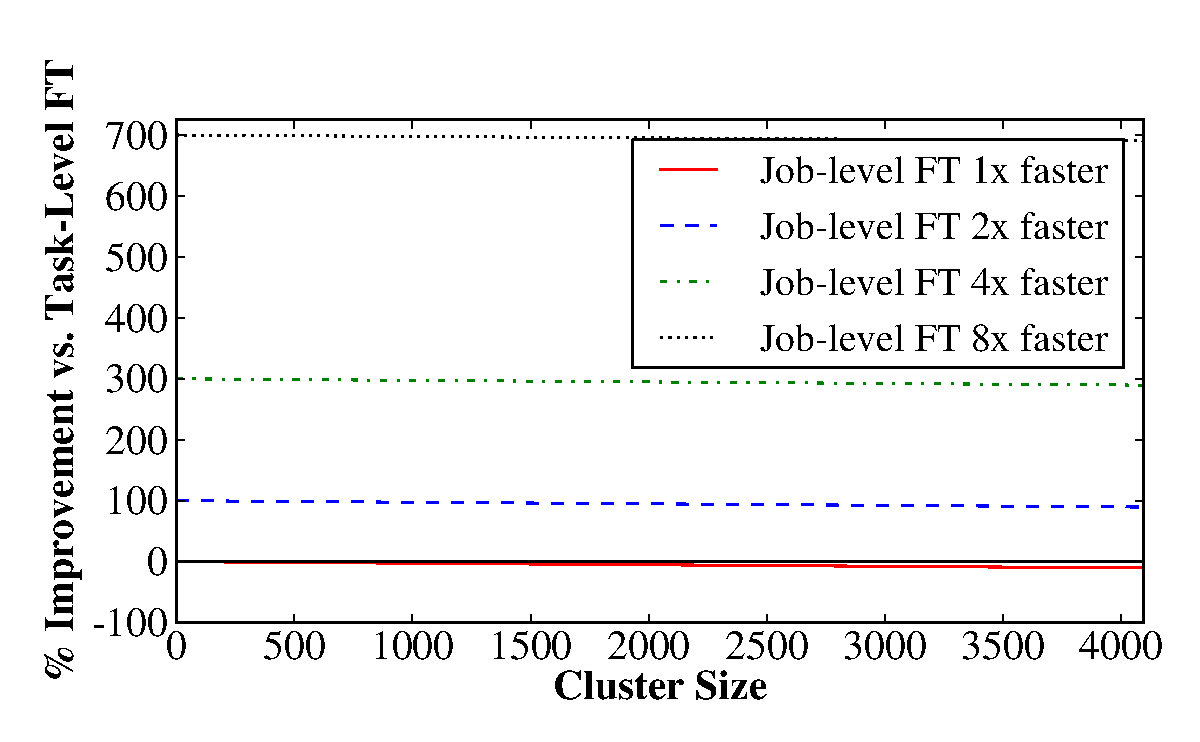
\includegraphics[width=\textwidth]{themis/graphs/analytical_failure_motivation/factor_5min}
  \caption{\label{fig:ft_motivation5} 5-minute job}
\end{subfigure}
\begin{subfigure}[t]{0.47\textwidth}
\centering
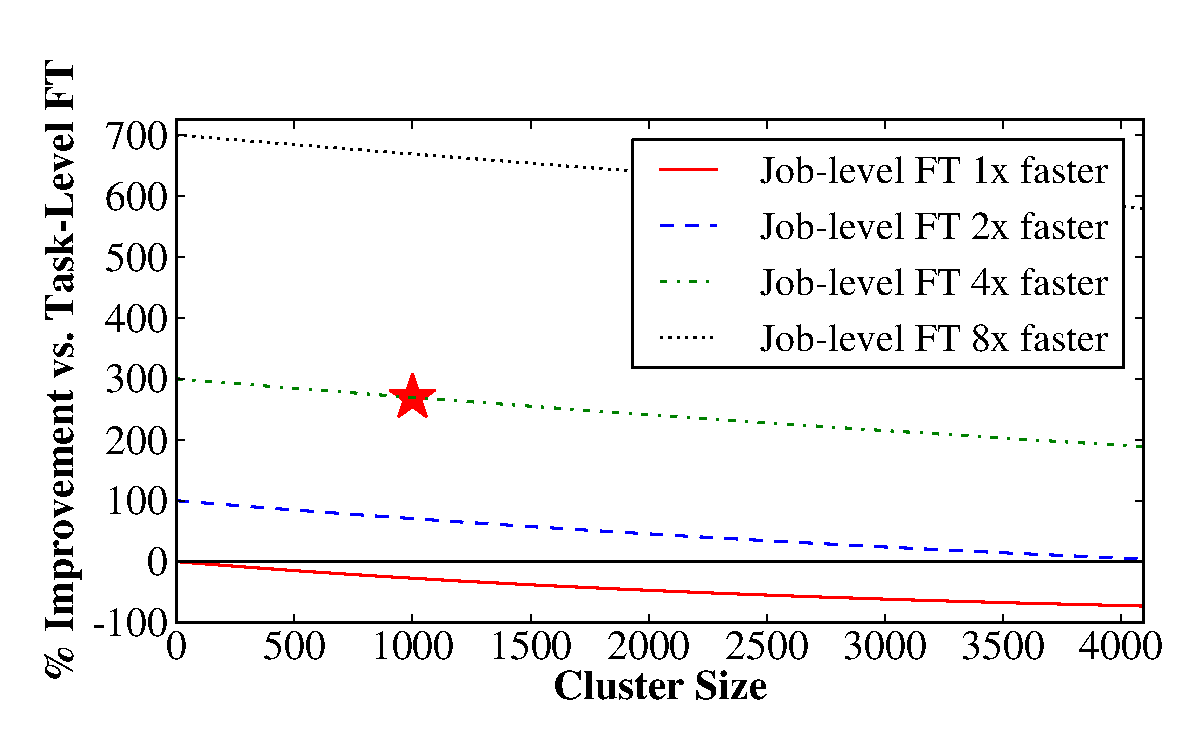
\includegraphics[width=\textwidth]{themis/graphs/analytical_failure_motivation/factor_60min}
\caption{\label{fig:ft_motivation60} 1-hour job (see text below for explanation of marked point)}
\end{subfigure}
\begin{subfigure}[t]{0.47\textwidth}
\centering
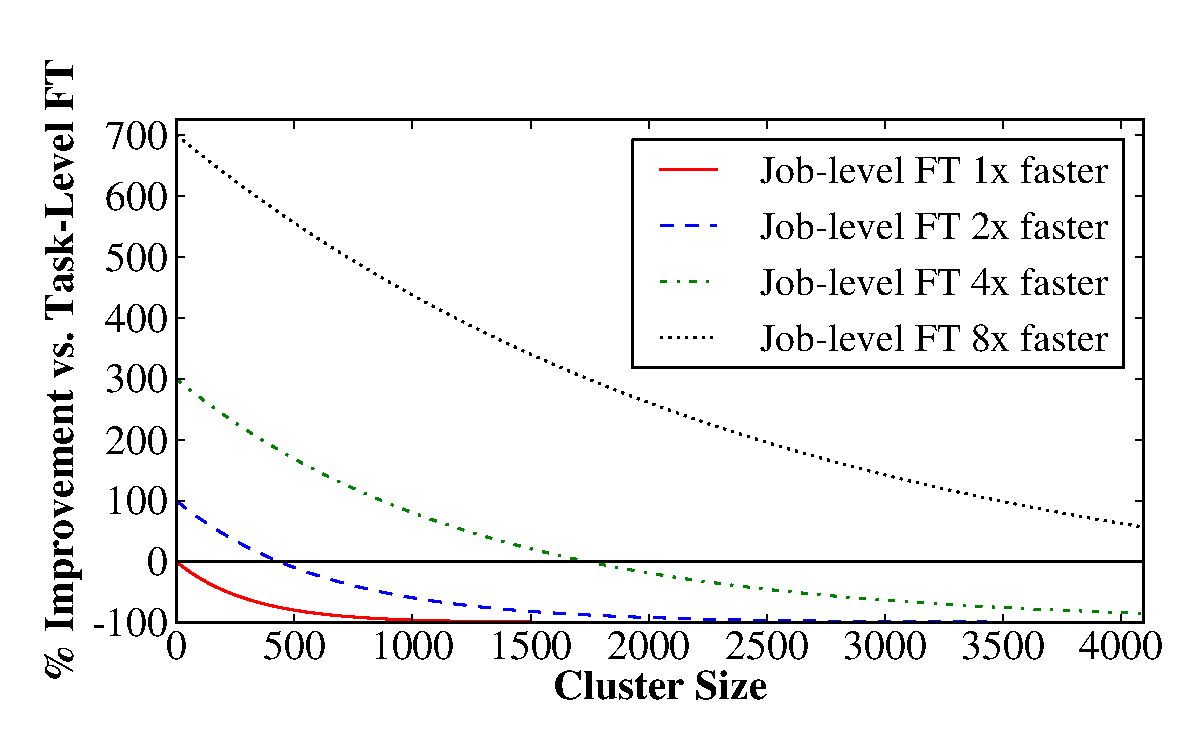
\includegraphics[width=\textwidth]{themis/graphs/analytical_failure_motivation/factor_600min}
\caption{\label{fig:ft_motivation600}10-hour job}
\end{subfigure}
\caption{\label{fig:ft_motivation} A lower-bound of the expected benefit of
  job-level fault tolerance for varying cluster sizes, given
  that an error-free execution of a job with task-level fault tolerance takes
  five minutes (\subref{fig:ft_motivation5}), an hour (\subref{fig:ft_motivation60}),
  or ten hours (\subref{fig:ft_motivation600}) to complete.}
\end{figure*}

Much of MapReduce's architecture is based on the assumption that it is running
on a very large cluster of unreliable machines.  However, a large number of
``Big Data'' clusters do not approach the size of warehouse-scale data centers
like those at Google and Microsoft because moderately-sized clusters (10s of
racks or fewer) are increasingly able to support important real-world problem
sizes.  The storage capacity and number of CPU cores in commodity servers are
both increasing rapidly.  In Cloudera's reference system
design~\cite{ClouderaDellHadoopPlatform}, in which each node has 16 or more
disks, a petabyte worth of 1TB drives fits into just over three racks, or about
60 nodes.  Coupled with the emergence of affordable 10 Gbps Ethernet at the end
host and increasing bus speeds, data can be packed more densely than ever
before while keeping disk I/O as the bottleneck resource.  This implies that
fewer servers are required for processing large amounts of data for I/O-bound
workloads.  We now consider the implications of this increased density on fault
tolerance.

Job-level fault tolerance allows for much more aggressive operator pipelining
than task-level fault tolerance can achieve while still maintaining the 2-IO
property.  However, it is not self-evident that the overhead of re-executing
failed jobs does not cancel any performance gained by this aggressive
pipelining.  In this section, we show not only that job-level fault tolerance
is a feasible approach for moderately-sized clusters, but also that there are
significant potential performance benefits for using job-level fault tolerance
in these environments.

\begin{table}
\centering
\caption{\label{tbl:googleMttf} Component-level failure rates
observed in a Google data center as reported
in~\cite{google-availability:osdi10}.}
\begin{tabular}{|c|c|} \hline
\textbf{Component} & \textbf{Failure rates}\\\hline
Node & 4.3 months \\
Disk & 2-4\% annualized\\
Rack & 10.2 years \\\hline
\end{tabular}
\end{table}

Understanding the expected impact of failures is critical to choosing the
appropriate fault tolerance model.  MapReduce was designed for clusters of many
thousands of machines running inexpensive, failure-prone commodity
hardware~\cite{mapreduce}.  For example, Table~\ref{tbl:googleMttf} shows
component-level mean-time to failure (MTTF) statistics in one of Google's data
centers~\cite{google-availability:osdi10}. Google's failure statistics are
corroborated by similar studies of hard
drive~\cite{DBLP:conf/fast/PinheiroWB07,Schroeder:2007:UDF:1288783.1288785} and
node~\cite{DBLP:conf/nsdi/NathYGS06, Schroeder:2010:LSF:1916484.1916652}
failure rates.

\subsection{Modeling Node Failure Rates}

At massive scale, there is a high probability that some portion of the cluster
will fail during the course of a job.  To understand this probability, we
employ a simple model~\cite{sysreliability}, shown in
Equation~\ref{eqn:jobfailure}, to compute the likelihood that a node in a
cluster of a particular size will experience a failure during a job:

\begin{equation}
P(N, t, MTTF) = 1 - e^{-N \cdot t / MTTF}
\label{eqn:jobfailure}
\end{equation}

The probability of a failure occurring in the next $t$ seconds is
a function of (1) the number of nodes in the cluster, $N$, (2) $t$, and (3) the
mean time to failure of each node, $MTTF$, taken from the node-level failure
rates in Table~\ref{tbl:googleMttf}.  This model assumes that nodes fail with
exponential (Pareto) probability, and we simplify our analysis by considering
node failures only.  We do this because disk failures can be made rare by using
node-level mechanisms (i.e., RAID), and correlated rack failures are likely to
cripple the performance of a cluster with only a few racks.

Based on the above model, in a 100,000 node data center, there is a 93\% chance
that a node will fail during any five-minute period. On the other hand, in a
moderately-sized cluster (e.g., 200 nodes, the average Hadoop cluster size as
reported by Cloudera), there is only a 0.53\% chance of encountering a node
failure during a five-minute window, assuming the MTTF rates in
Table~\ref{tbl:googleMttf}.

This leads to the question of whether smaller deployments benefit from
job-level fault tolerance, where if any node running a job fails the entire job
restarts.  Intuitively, this scheme will be more efficient overall when
failures are rare and/or jobs are short.

\subsection{Modeling Expected Job Completion Time}

Let $T$ be the job's duration and $MTTF$ be the mean time to failure of the
cluster. In our model, failure occurs as a Poisson process. We compute the
expected running time of a failed job (denoted $T_F$) as follows:

\vspace{-4mm}

\begin{eqnarray}
T_{F} &=& \int_{0}^{T} t \cdot \frac{1}{MTTF} e^{-\frac{t}{MTTF}} dt \notag \\
      &=& \left[- t e^{-\frac{t}{MTTF}} - MTTF \cdot e^{-\frac{t}{MTTF}}\right]_{t = 0}^{t = T} \notag \\
      &=& MTTF - (T + MTTF) e^{-\frac{T}{MTTF}}
\label{eqn:T_F}
\end{eqnarray}

Therefore, if the job duration $T$ is much larger than the MTTF of the cluster
($T \gg MTTF$), Equation~\ref{eqn:T_F} implies that $T_F \approx MTTF$, and we
expect the job to fail. On the other hand, if $T \ll MTTF$,
Equation~\ref{eqn:T_F} implies that $T_F \approx T$, and we expect the job to
succeed.

Having modeled the running time of a failed job, we can now derive a model for
overall job completion time. Let $p$ denote the probability of failure in a
single Themis job.  Let $T$ denote the running time of the job when there are
no failures.

Consider a situation in which the job fails during the first $(n-1)$ trials and
completes in the $n^{th}$ trial. The probability of this event is $p^{n-1} (1 -
p)$.  Note that a successful trial takes time $T$ and a failed trial takes time
$T_F$.  To simplify our notation, let $\alpha = T_F / T$ be the fraction of its
successful runtime the failed job spent running.  Then the total running time
in this case is
\[(n-1) \alpha T + T = ((n-1) \alpha + 1) T.\]

By considering such an event for all possible values of $n$, we get the
expected running time to completion for the job:

\vspace{-4mm}

\begin{eqnarray}
   S(p, T) &=& \sum_{n=1}^{\infty} ((n-1) \alpha + 1) T \cdot p^{n-1}(1-p)  \notag \\
           &=& T(1-p) \sum_{n=1}^{\infty} \left(\alpha n p^{n-1} + (1-\alpha) p^{n-1}\right)  \notag \\
           &=& T(1-p) \left(\alpha \sum_{n=1}^{\infty} n p^{n-1} + (1 - \alpha) \sum_{n=1}^{\infty} p^{n-1}\right) \notag \\
           &=& T(1-p) \left(\alpha \frac{1}{(1-p)^2} + (1 - \alpha) \frac{1}{1-p}\right) \notag \\
           &=& T \left(\alpha \frac{p}{1-p} + 1\right)
\label{eqn:job}
\end{eqnarray}

Hence, we can model the expected completion time of a job $S(p,T)$ as:

\begin{equation}
S(p,T) = T\left(\frac{p}{1 - p} + 1\right)
\label{eqn:expectedjobtime}
\end{equation}

where $p$ is the probability of a node in the cluster failing, and $T$ is the
runtime of the job.  This estimate is pessimistic, in that it assumes that jobs
fail just before the end of their execution.

By combining equations~\ref{eqn:jobfailure} and \ref{eqn:expectedjobtime}, we
can compute the expected benefit--or penalty--that we get by moving to
job-level fault tolerance.  Modeling the expected runtime of a job with
task-level fault tolerance is non-trivial, so we instead compare to an
error-free baseline in which the system's performance is not affected by node
failure.  This comparison underestimates the benefit of job-level fault
tolerance.

Figure~\ref{fig:ft_motivation} shows the expected performance benefits of
job-level fault tolerance compared to the error-free baseline.  More formally,
we measure performance benefit as $S(P(\cdot),T_{job}) / T_{task}$,
where $T_{job}$ is the time a job on an error-free cluster takes to execute
with job-level fault tolerance and $T_{task}$ is the time the same job takes to
execute with task-level fault tolerance.

The benefits of job-level fault tolerance increase as the error-free
performance improvement made possible by moving to job-level fault tolerance
(i.e. $T_{task} / T_{job}$) increases. For example, if $T_{task} / T_{job}$ is
4, $T_{task}$ is one hour and we run on a cluster of 1,000 nodes, we can expect
\themis to complete the job 240\% faster than the task-level fault tolerant
alternative on average; this scenario is marked with a star in
Figure~\ref{fig:ft_motivation60}.  There are also situations in which
job-level fault tolerance will significantly under-perform task-level fault
tolerance.  For example, if $T_{task} / T_{job}$ is 2, \themis will
under-perform a system with task-level fault tolerance for clusters bigger than
500 nodes.  From this, we make two key observations: for job-level fault
tolerance to be advantageous, the cluster has to be moderately-sized, and
\themis must significantly outperform the task-level alternative.
